% Faddeev-Skyrme soliton energies from controlled lattice extrapolation
% Build:  pdflatex -> bibtex -> pdflatex -> pdflatex   (see build.sh)

\documentclass[aps,prd,preprint,nofootinbib,longbibliography]{revtex4-2}

\usepackage{amsmath}
\usepackage{amssymb}
\usepackage{bm}
\usepackage{graphicx}
\usepackage[colorlinks=true,linkcolor=blue,citecolor=blue,urlcolor=blue]{hyperref}

\raggedbottom
\newcommand{\nv}{\bm{n}}
\newcommand{\Av}{\bm{A}}
\newcommand{\Bv}{\bm{B}}
\newcommand{\Qh}{Q_H}
\newcommand{\Ehat}{\hat{E}}
\newcommand{\Rhat}{\hat{R}}

\begin{document}

\title{Faddeev--Skyrme soliton energies\\ from controlled lattice extrapolation}

\author{Paul Vodrazka}
\affiliation{Independent researcher}
\date{\today}

\begin{abstract}
We recompute the charge-one Faddeev--Skyrme soliton energy with both lattice
systematics under explicit control and obtain $E_1/c_0=1.231\pm0.003$, an excess
of $2.2\%$ over the accepted $1.204$ that we have been unable to remove. The
systematics matter because they act in opposite directions---finite spacing
lowers the energy, a finite periodic box raises it---so neither can be assessed
alone; fitting $E=E_\infty-ah^2+cL^{-p}$ to nine runs separates them. Three
checks bear on whether the fault is ours. At matched spacing $h=0.100$, the grid
of the reference computation, we obtain $1.2257$ with no extrapolation, a
$1.8\%$ gap of which our finite box can account for at most $0.7\%$. A
fourth-order accurate symmetrisation, whose error has the opposite sign,
extrapolates from above to $1.2371$ against the second-order scheme's $1.2354$
from below, the two agreeing to $0.14\%$. And the identical procedure applied to
the Skyrme model, where the charge-one energy follows from an ordinary
differential equation, recovers that exact value to $0.03\%$ from runs whose
individual errors reach $2\%$. The discrepancy is confined to the absolute
normalisation: we reproduce the published charge-one to charge-four
configuration types, the scaling exponent $0.765$ against $3/4$, binding against
fission in every sector, and, in the frame sector, binding energies per baryon
within $0.15$ percentage points of the tabulated values. We also record a
discretisation pitfall with consequences beyond bookkeeping: any derivative
whose symbol vanishes at the Nyquist frequency gives the discrete energy exact
flat directions, along which the topological charge unwinds at no cost and the
energy falls below the Vakulenko--Kapitanskii bound.
\end{abstract}

\maketitle

\section{Introduction}
\label{sec:intro}

The Faddeev--Skyrme model~\cite{faddeev1999} is the simplest field theory in
three dimensions whose solitons are classified by a linking number rather than a
winding number. For a unit three-vector field $\nv:\mathbb{R}^3\to S^2$ with
$\nv\to\nv_0$ at infinity, configurations fall into sectors labelled by the Hopf
invariant $\Qh\in\pi_3(S^2)=\mathbb{Z}$, and the minimal energy in each sector is
a well-posed numerical question that has been studied for two
decades~\cite{faddeev1997,gladikowski1997,battye1998,hietarinta1999,ward1999,sutcliffe2007}.
The charge-one energy is the reference against which all other sectors are
quoted, and it is usually taken to be $1.204$ in the normalisation fixed by
Ward's conjectured bound.

This paper recomputes that number with the two lattice systematics separated and
extrapolated, and reports that we cannot reproduce it. Our value is $2.2\%$
higher. Because a discrepancy of this size is more often a defect of the
computation than of the literature, most of what follows is an attempt to break
our own result.

Two things make the exercise worth reporting. The first is a discretisation
pitfall that is easy to fall into and whose symptom is dramatic---the topological
charge simply dissolves---but which we have not seen stated in these terms. The
second is that the two lattice systematics push in opposite directions, so a
study that varies only the spacing, or only the box, will appear better converged
than it is. Section~\ref{sec:lattice} treats the first,
Section~\ref{sec:charge1} the second.

Section~\ref{sec:frame} is the control. Applied to the Skyrme model, where the
charge-one energy is available from an ordinary differential equation, the same
code and the same extrapolation recover the exact answer to three parts in ten
thousand. Section~\ref{sec:spectrum} reports the $\Qh\le4$ spectrum, which
agrees with the published one in every structural respect. All source is
available~\cite{repo}.

\section{Model, bound and normalisation}
\label{sec:model}

The static energy is
\begin{equation}
E[\nv]=\int d^3x\,\Big[c_2\,\partial_i\nv\cdot\partial_i\nv
 + \tfrac{c_4}{2}\,(\partial_i\nv\times\partial_j\nv)\cdot
 (\partial_i\nv\times\partial_j\nv)\Big],
\label{eq:fs}
\end{equation}
and we set $c_2=c_4=1$ throughout, so that lengths and energies are in model
units. Under $\nv(x)\to\nv(x/\mu)$ the two terms scale as
$E(\mu)=\mu E_2+\mu^{-1}E_4$, so every stationary point satisfies the virial
identity $E_2=E_4$; with either constant absent the soliton collapses or spreads,
and Derrick's theorem is satisfied rather than evaded.

Finite-energy configurations obey the bound of Vakulenko and
Kapitanskii~\cite{vakulenko1979},
\begin{equation}
E\ge c_0|\Qh|^{3/4},
\end{equation}
whose proof does not fix the constant. Ward~\cite{ward1999} conjectured the sharp
value, which in the normalisation of~\eqref{eq:fs} reads
\begin{equation}
c_0=32\pi^2\sqrt{2}=446.65 .
\label{eq:c0}
\end{equation}
Reference~\cite{sutcliffe2007} divides its energies by exactly this factor and
states the conjecture with unit coefficient; its integrand is identical
to~\eqref{eq:fs}, so its tabulated energies are directly comparable with ours
with no conversion. We have verified the identity
$\tfrac12(\partial_i\nv\times\partial_j\nv)^2
=\tfrac12[(\partial_i\nv\cdot\partial_i\nv)^2
-(\partial_i\nv\cdot\partial_j\nv)^2]$ symbolically, so the two normalisations
agree term by term.

Because the exponent $3/4$ is sub-linear, $E_Q<|Q|E_1$ is permitted and
multi-charge solitons may be bound against fission; whether they are is settled
in Sec.~\ref{sec:spectrum}. For the general theory we refer to Manton and
Sutcliffe~\cite{mantonsutcliffe2004}.

\section{Lattice construction, and a null mode that destroys topology}
\label{sec:lattice}

We minimise~\eqref{eq:fs} on a periodic cubic lattice. One implementation choice
carries more than numerical significance.

With central differences \emph{of any order}, the Fourier symbol of the
derivative operator vanishes at the Nyquist wavenumber. For the fourth-order
antisymmetric stencil, setting $f_{i\pm1}\to-f_i$ and
$f_{i\pm2}\to f_i$ gives identically zero. A checkerboard mode therefore costs
\emph{no energy}. The discrete energy acquires exact flat directions, and
gradient flow carries any Hopfion monotonically to the vacuum: in our first runs
$\Qh$ fell from $1$ to $0$ while $E$ fell far below the bound $c_0|\Qh|^{3/4}$,
which is supposed to be inviolable. The topological protection is
lost not because the physics permits it but because the discretisation has a
zero-cost path out of the sector.

The cure is a scheme whose symbol vanishes only at $k=0$. We use one-sided
differences and symmetrise the \emph{energy} rather than the derivative,
\begin{equation}
E=\tfrac12\big[E(D^+\nv)+E(D^-\nv)\big],\qquad
(D^\pm f)_i=\pm\frac{f_{i\pm1}-f_i}{h},
\label{eq:sym}
\end{equation}
which has no null mode and, because $(D^\pm)^{\mathsf T}=-D^\mp$ holds exactly on
a periodic lattice, makes the analytic variation the \emph{exact} gradient of the
discrete energy. We verify this against finite differences of the energy density
to a maximum relative error of $5\times10^{-7}$.

The symmetrisation also fixes the form of the extrapolation used below. Expanding
$D^\pm_i=\partial_i\pm\tfrac{h}{2}\partial_i^2+\tfrac{h^2}{6}\partial_i^3+\ldots$
and averaging removes the $O(h)$ term, leaving
\begin{equation}
\tfrac12\!\int\!\big[|D^+\nv|^2+|D^-\nv|^2\big]
 = \int\!|\partial\nv|^2 - \frac{h^2}{12}\int\!|\partial^2\nv|^2 + O(h^4),
\label{eq:h2}
\end{equation}
after integrating $\int\partial\nv\cdot\partial^3\nv=-\int|\partial^2\nv|^2$ by
parts. The discrete energy is therefore below the continuum one, by $O(h^2)$ --
both the sign and the order seen in the fits of Sec.~\ref{sec:charge1}.

\emph{A fourth-order variant.} Nothing forces the one-sided differences
in~\eqref{eq:sym} to be first-order accurate. Built from third-order one-sided
differences,
\begin{equation}
(D^+_3f)_i=\frac{-11f_i+18f_{i+1}-9f_{i+2}+2f_{i+3}}{6h},
\end{equation}
and its reflection, the leading errors are equal and opposite,
$D^\pm_3=\partial\pm\tfrac{h^3}{4}\partial^4+\ldots$, so they cancel in the
symmetrised energy and leave an $O(h^4)$ scheme. Its Nyquist symbol is $-20/3h$
rather than zero, so the null mode is still absent, and
$(D^+_3)^{\mathsf T}=-D^-_3$ still holds, so the variation remains exact. We
refer to the two schemes as $O(h^2)$ and $O(h^4)$; crucially their errors have
opposite sign, so together they bracket the continuum limit.

The Hopf charge is evaluated by reconstructing $\Av$ spectrally in Coulomb gauge
from $\Bv$, with $\|\nabla\times\Av-\Bv\|/\|\Bv\|<10^{-4}$. Seeds of known charge
come from composing a degree-$d$ hedgehog with the Hopf projection (giving
$\Qh=d$, since the Chern--Simons three-form pulls back with the degree) and from
the toroidal $A_{n,m}$ ansatz~\cite{gladikowski1997,hietarinta1999} (giving
$\Qh=nm$).

\section{The charge-one energy}
\label{sec:charge1}

Two systematics act in opposite directions, and both must be removed before any
comparison is meaningful.

\emph{Finite spacing lowers the energy}, by~\eqref{eq:h2}. Repeating the $\Qh=1$
relaxation at fixed box $L=12$, with every lattice initialised by resampling the
converged solution so that all points share the same convergence quality, gives
Table~\ref{tab:hconv}. The measured charge approaches the integer and the virial
ratio approaches unity, both as they must.

\begin{table}[t]
\caption{Lattice-spacing dependence of the $\Qh=1$ soliton at $L=12$.}
\label{tab:hconv}
\begin{ruledtabular}
\begin{tabular}{cccccc}
$N$ & $h$ & $E$ & $E/c_0$ & $\Qh$ & $E_2/E_4$ \\
\colrule
 56 & 0.2143 & 532.28 & 1.1917 & 0.9833 & 0.823 \\
 72 & 0.1667 & 540.42 & 1.2100 & 0.9951 & 0.883 \\
 88 & 0.1364 & 544.12 & 1.2182 & 0.9980 & 0.904 \\
 96 & 0.1250 & 545.29 & 1.2208 & 0.9986 & 0.908 \\
104 & 0.1154 & 546.18 & 1.2228 & 0.9990 & 0.910 \\
120 & 0.1000 & 547.45 & 1.2257 & 0.9994 & 0.911 \\
\end{tabular}
\end{ruledtabular}
\end{table}

\emph{Finite volume raises it.} The director is massless, so the soliton has
power-law tails and interacts with its own periodic images. Holding $h=1/6$ and
enlarging the box gives $E=540.50,\,538.77,\,538.40$ for $L=12,16,20$, with the
energy fraction within six cells of the boundary falling from
$4.0\times10^{-3}$ to $1.3\times10^{-4}$.

Neither series alone is a convergence test, because the two effects partially
cancel. Fitting them together,
\begin{equation}
\frac{E}{c_0} = E_\infty - a\,h^2 + c\,L^{-p},
\label{eq:extrap}
\end{equation}
to all nine runs gives an $h^2$ coefficient $a=0.94$, a box correction of $+0.4$
to $+0.7\%$ at $L=12$, and
\begin{equation}
E_1 = 550\pm2, \qquad E_1/c_0 = 1.231\pm0.003 ,
\label{eq:e1}
\end{equation}
with residuals of $4\times10^{-4}$ throughout. The quoted spread is the variation
of the intercept as the box exponent is fixed anywhere between $p=2$ and $p=6$,
widened to cover a second fit to an independently relaxed set of runs. The
extrapolation reaches only $0.4\%$ beyond the finest lattice computed.

Against the published $1.204$ this is an excess of $2.2\%$. Three checks bear on
whether the fault is ours.

\emph{Matched resolution.} Our finest lattice uses $h=0.100$, exactly the spacing
of Ref.~\cite{sutcliffe2007}, and returns $1.2257$ with no extrapolation at all.
At equal spacing the gap is $1.8\%$, of which our finite box can account for at
most $0.7\%$.

\emph{An independent discretisation.} The remaining worry is that our energy is
only $O(h^2)$ accurate while Ref.~\cite{sutcliffe2007} uses fourth-order
derivatives, so that the extrapolation rather than the data is at fault. Repeating
the whole calculation with the $O(h^4)$ scheme of Sec.~\ref{sec:lattice}, whose
error enters with the opposite sign, gives Table~\ref{tab:o4}: the two schemes
approach from opposite sides and agree with each other to $0.14\%$. Two
discretisations of different order converging from opposite directions do not
conspire.

\begin{table}[t]
\caption{The two symmetrised schemes at $L=12$. The $O(h^2)$ scheme approaches
from below and the $O(h^4)$ scheme from above; the extrapolations agree to
$0.14\%$. Values are $E/c_0$ before the box correction of
Eq.~\eqref{eq:extrap}.}
\label{tab:o4}
\begin{ruledtabular}
\begin{tabular}{ccccc}
$h$ & $O(h^2)$ & $E_2/E_4$ & $O(h^4)$ & $E_2/E_4$ \\
\colrule
0.1875 & 1.2026 & 0.862 & 1.2646 & 1.071 \\
0.1500 & 1.2147 & 0.902 & 1.2492 & 0.975 \\
0.1250 & 1.2207 & 0.920 & 1.2420 & 0.943 \\
\colrule
$\to0$ & \textbf{1.2354} & & \textbf{1.2371} & \\
\end{tabular}
\end{ruledtabular}
\end{table}

\emph{A control with a known answer.} This is Sec.~\ref{sec:frame}.

\section{A control: the frame sector}
\label{sec:frame}

The Faddeev--Skyrme model has no closed-form solution, so within it a lattice can
only be compared against other lattices. The Skyrme model does have one, and it
is close enough to be a genuine control: the same energy functional, the same
code, the same boundary conditions and the same extrapolation, with only the
target changed from $S^2$ to $S^3$.

For $\varphi:\mathbb{R}^3\to S^3$ the energy~\eqref{eq:fs} is the Skyrme
model~\cite{skyrme1961} in Manton's strain form~\cite{manton1987}, configurations
are classified by $\pi_3(S^3)=\mathbb{Z}$ with baryon number
\begin{equation}
B=\frac{1}{2\pi^2}\int
\det\!\left[\varphi,\partial_1\varphi,\partial_2\varphi,\partial_3\varphi\right]d^3x,
\end{equation}
and the topological bound follows from two applications of AM--GM to the
principal stretches, $E\ge12\pi^2\sqrt{c_2c_4}\,|B|$. For $B=1$ the minimiser is
spherically symmetric, so with $\varphi=(\cos f,\sin f\,\hat{\bm r})$ the energy
reduces to
\begin{equation}
E = 4\pi\!\int_0^\infty\!\!\left[f'^2r^2 + 2\sin^2\!f\,(1+f'^2)
 + \frac{\sin^4\!f}{r^2}\right]dr ,
\end{equation}
whose Euler--Lagrange equation we solve as a two-point boundary value problem
with $f(0)=\pi$, $f(\infty)=0$, obtaining
\begin{equation}
E/12\pi^2 = 1.23145 ,
\label{eq:ode}
\end{equation}
consistent with the value $1.232$ standard since Ref.~\cite{adkins1983}. Because
we compute~\eqref{eq:ode} ourselves it tests the lattice rather than our reading
of a table.

Relaxing on the lattice at two box sizes and three spacings each, and fitting
Eq.~\eqref{eq:extrap} to all six runs, gives
\begin{equation}
E_\infty/12\pi^2 = 1.2311 ,
\end{equation}
with an rms residual of $6.5\times10^{-5}$ and a leave-one-out spread of
$\pm0.0008$. This is $0.03\%$ from the exact answer~\eqref{eq:ode}, obtained from
runs whose individual errors reach $2\%$. The box exponent comes out
$p\simeq2.2$, and the $L=8$ series overshoots the exact value while still rising
with resolution---direct confirmation that a periodic box biases upward, an
effect also noted in the Skyrme literature~\cite{battye2002}.

A procedure accurate to three parts in ten thousand on a problem with a known
answer is unlikely to be wrong by $2\%$ on a neighbouring one. This is our main
reason for reporting the discrepancy of Sec.~\ref{sec:charge1} as a discrepancy.

The same machinery reproduces the multi-baryon sector.
Table~\ref{tab:frame} gives $B=1$--$4$ from symmetric rational-map
seeds~\cite{houghton1998}; the energies sit $0.6$--$0.8\%$ below the tabulated
values~\cite{battye2002}, uniformly, so the binding energies---being ratios, in
which the systematic cancels---come out within $0.15$ percentage points.

\begin{table}[t]
\caption{Frame-sector solitons at $L=12$, $N=96$, from rational-map seeds of the
indicated symmetry. Literature values are Ref.~\cite{battye2002}. Binding is
$1-E_B/(B E_1)$.}
\label{tab:frame}
\begin{ruledtabular}
\begin{tabular}{cccccc}
$B$ & symmetry & $E/12\pi^2B$ & Ref.~\cite{battye2002} & binding & lit.\ binding \\
\colrule
1 & spherical    & 1.2231 & 1.2322 & ---     & --- \\
2 & axial        & 1.1712 & 1.1791 & $4.25\%$ & $4.31\%$ \\
3 & tetrahedral  & 1.1396 & 1.1462 & $6.83\%$ & $6.98\%$ \\
4 & cubic        & 1.1110 & 1.1201 & $9.17\%$ & $9.10\%$ \\
\end{tabular}
\end{ruledtabular}
\end{table}

\section{The charge-one to charge-four spectrum}
\label{sec:spectrum}

Table~\ref{tab:spectrum} gives the Hopf spectrum on a common lattice, and
Table~\ref{tab:validation} compares it with Ref.~\cite{sutcliffe2007};
Fig.~\ref{fig:structure} shows the relaxed configurations and
Fig.~\ref{fig:spectrum} the energies against the bound and the fission
threshold.

\begin{figure}[t]
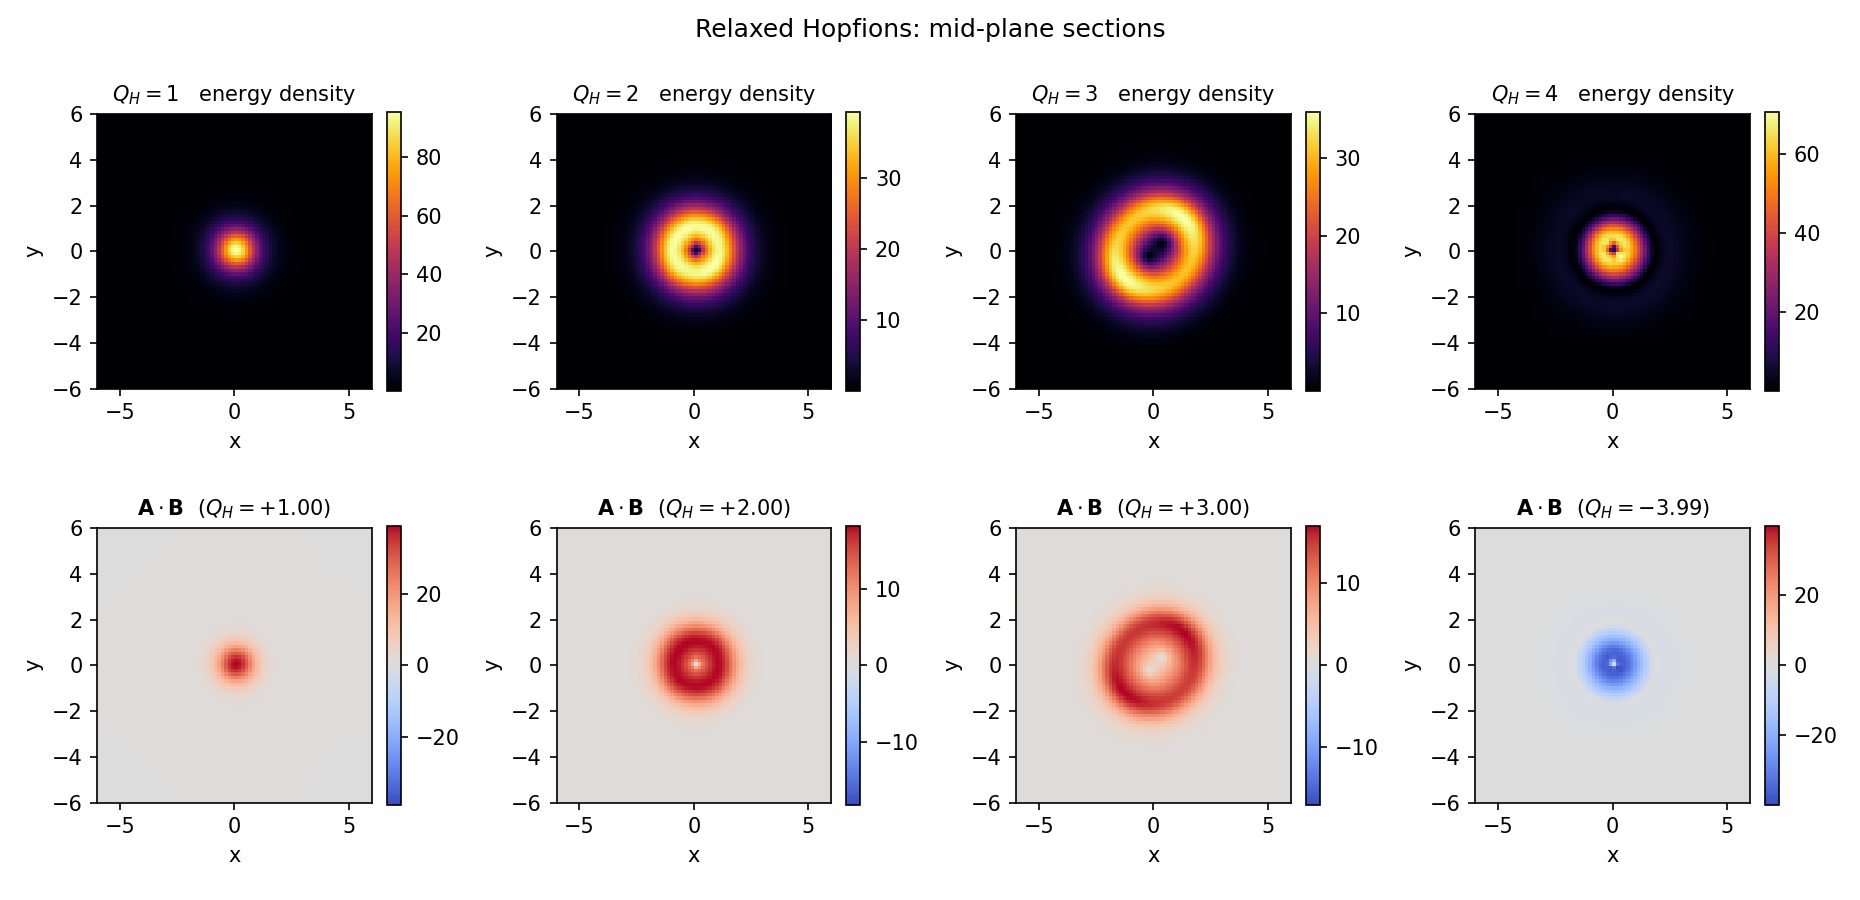
\includegraphics[width=\columnwidth]{../../figures/hopfion_structure.png}
\caption{Mid-plane sections of the relaxed Hopfions. Top: energy density.
Bottom: Hopf density $\Av\cdot\Bv$ on a symmetric colour scale, so the vacuum is
neutral in every panel; the $\Qh=4$ solution was found with negative charge,
which is equivalent to the positive one by a spatial reflection. The $\Qh=2,3$
ground states are toroidal; the $\Qh=4$ ground state is the more compact linked
$A_{2,2}$ configuration.}
\label{fig:structure}
\end{figure}

\begin{figure}[t]
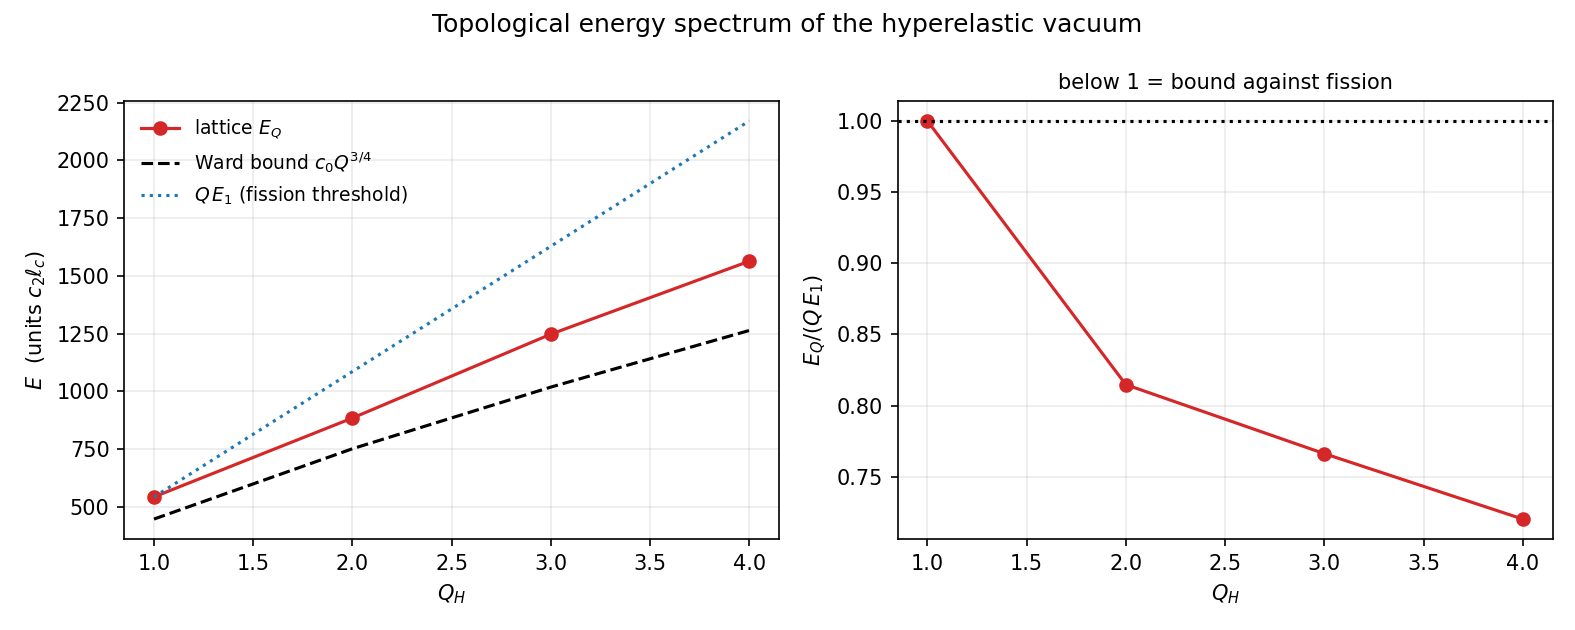
\includegraphics[width=\columnwidth]{../../figures/energy_spectrum.png}
\caption{Left: computed energies against the Ward bound $c_0Q^{3/4}$ and the
fission threshold $QE_1$. Right: $E_Q/(QE_1)$; values below unity indicate
binding against fission.}
\label{fig:spectrum}
\end{figure}

\begin{table}[t]
\caption{Relaxed Hopfion spectrum ($N=80$, $L=12$, $h=0.15$). Several
independent seeds were relaxed in each sector and the lowest is quoted.}
\label{tab:spectrum}
\begin{ruledtabular}
\begin{tabular}{ccccccc}
$\Qh$ & seed & $E$ & $E/c_0|Q|^{3/4}$ & $R_{\rm rms}$ & $E_2/E_4$ & $E_Q/(QE_1)$ \\
\colrule
1 & hedgehog $d{=}1$ & 542.65  & 1.215 & 1.705 & 0.887 & 1.000 \\
2 & hedgehog $d{=}2$ & 884.15  & 1.177 & 2.089 & 0.950 & 0.815 \\
3 & hedgehog $d{=}3$ & 1247.30 & 1.225 & 2.489 & 0.955 & 0.766 \\
4 & $A_{2,2}$ (linked) & 1563.24 & 1.237 & 2.331 & 0.956 & 0.720 \\
\end{tabular}
\end{ruledtabular}
\end{table}

\begin{table}[t]
\caption{Comparison with Ref.~\cite{sutcliffe2007} in the common normalisation
$E/c_0$, on the lattice of Table~\ref{tab:spectrum}. The ground-state
configuration type is reproduced in every sector.}
\label{tab:validation}
\begin{ruledtabular}
\begin{tabular}{ccccc}
$\Qh$ & this work & Ref.~\cite{sutcliffe2007} & difference & type (ours / published) \\
\colrule
1 & 1.215 & 1.204 & $+0.9\%$ & $A_{1,1}$ / $A_{1,1}$ \\
2 & 1.980 & 1.967 & $+0.6\%$ & $A_{2,1}$ / $A_{2,1}$ \\
3 & 2.793 & 2.754 & $+1.4\%$ & $A_{3,1}$ / $\widetilde{A}_{3,1}$ \\
4 & 3.500 & 3.445 & $+1.6\%$ & $A_{2,2}$ / $A_{2,2}$ \\
\end{tabular}
\end{ruledtabular}
\end{table}

Four structural results, none of them imposed.

\emph{Every multi-charge sector is bound against fission}, $E_Q<QE_1$ by
$18.5\%$, $23.4\%$ and $28.0\%$ for $Q=2,3,4$.

\emph{The sub-linear exponent is recovered.} A power-law fit gives
$E_Q\propto|\Qh|^{0.765}$ against the Vakulenko--Kapitanskii $3/4$; the same fit
to the published energies gives $0.760$.

\emph{The $\Qh=4$ ground state is linked.} The $A_{2,2}$ seed relaxes to
$1563.2$, below both the hedgehog $d{=}4$ ($1621.6$) and $A_{4,1}$ ($1621.8$),
and it is more compact than the $\Qh=3$ soliton ($R_{\rm rms}=2.33$ against
$2.49$). Linking, not size, lowers the energy.

\emph{Seeds that should agree do.} $A_{2,1}\to884.20$ against the hedgehog's
$884.15$, and $A_{3,1}\to1248.34$ against $1247.30$: agreement at the $10^{-3}$
level from entirely different initial data. The $A_{1,m}$ family stalls higher
($1006.9$, $1478.9$, $1898.9$), which we report as upper stationary
configurations without claiming they are local minima.

The excess over Ward's bound is $21.5$, $17.7$, $22.5$ and $23.7\%$ here against
$20.4$, $17.0$, $20.8$ and $21.8\%$ in Ref.~\cite{sutcliffe2007}: not only the
overall $\sim20\%$ level but the characteristic dip at $\Qh=2$ is reproduced. The
structure of the spectrum is therefore not in question; the disagreement is
confined to the absolute normalisation.

\section{Discussion}

We are unable to reduce the charge-one discrepancy below $2\%$, and we have not
found a defect in our own calculation that would produce it. The candidate
explanations we can test have been tested: the spacing, by matching
Ref.~\cite{sutcliffe2007} exactly; the order of the scheme, by an independent
$O(h^4)$ discretisation approaching from the other side; the box, by an explicit
two-parameter fit; and the whole procedure, by a control with an exact answer.

What we cannot test from here is the effect of fixed rather than periodic
boundaries, which is the one methodological difference remaining.
Reference~\cite{sutcliffe2007} truncates the field to the vacuum at the boundary
of a box of side $15.1$; for a massless field with power-law tails this removes
gradient energy that a periodic box retains, and the sign is right to explain
part of a gap. Against that, Ref.~\cite{sutcliffe2007} itself argues the opposite
way, noting that its grid ``appear[s] to underestimate the energy by an amount of
the order of $1\%$'' and quoting $E\simeq1.21$ from higher-resolution studies.
Our result would put the underestimate nearer $2\%$.

The cleanest resolution would be an independent computation with fixed boundaries
and an $h\to0$ extrapolation, which we encourage; the code needed to reproduce
everything here, including both schemes, is available~\cite{repo}. Until then we
report $E_1/c_0=1.231\pm0.003$ as our result and the difference from $1.204$ as
open.

\begin{acknowledgments}
Numerical work used NumPy, SciPy, SymPy, Matplotlib and CuPy. The author used an
AI assistant (GitHub Copilot) for code development, numerical analysis and
manuscript preparation; all claims, and responsibility for them, are the
author's.
\end{acknowledgments}

\appendix

\section{Numerical methods}

\emph{Discretisation.} Periodic cubic lattice; the energy is the symmetrisation
of Eq.~\eqref{eq:sym} in either the $O(h^2)$ or the $O(h^4)$ form. Because
$(D^\pm)^{\mathsf T}=-D^\mp$, the analytic variation is the exact gradient of the
discrete energy, verified against finite differences of the energy density to
$5\times10^{-7}$.

\emph{Minimisation.} Adaptive damped flow: the step is capped so that no site
rotates by more than $\delta$ radians per iteration; a heavy-ball term with
energy arrest accelerates convergence; and the momentum is projected back onto
the tangent space each step---omitting this projection allows a spurious radial
component to accumulate and drives the field out of its sector. Every hundred
steps the exact Derrick dilation $\mu=\sqrt{E_4/E_2}$ is applied and accepted
only if it lowers the energy \emph{and} does not push the configuration into the
boundary collar; the second condition matters, because unbounded dilation samples
only the core and returns a uniform field, whose energy is zero and which the
energy test alone would therefore accept.

\emph{Convergence.} Stationarity is checked by continued relaxation: the stored
$\Qh=1$ field moves by $2\times10^{-4}$ in relative energy over $1800$ further
steps, and the residual virial deficit is a property of the discrete functional
rather than of incomplete relaxation, since it persists while the energy is
stationary and falls with both $h$ and $L$.

\emph{Topological charge.} $\Bv$ from fourth-order central differences, $\Av$
from $\hat{\Av}=i\bm{k}\times\hat{\Bv}/k^2$ in Coulomb gauge; the residual
$\|\nabla\times\Av-\Bv\|/\|\Bv\|$ is below $10^{-4}$ at $N=96$. The baryon number
of the frame sector is the determinant of
$[\varphi,\partial_1\varphi,\partial_2\varphi,\partial_3\varphi]$ evaluated at
every site, and is integral to $5\times10^{-4}$ at the finest lattice.

\section{Reproducibility}

The supplement~\cite{repo} comprises a library and one driver per result, with
\texttt{verify\_claims.py} re-deriving every quoted quantity from the stored
fields rather than from intermediate summaries, and
\texttt{verify\_manuscript.py} checking that the numbers printed in this paper
are the numbers those drivers produced.
The lattice kernels are written against a swappable array backend and run unchanged
on a CPU or, with \texttt{-{}-gpu}, on a CUDA device; double precision is used
throughout, since the kernels are limited by memory bandwidth rather than by
floating-point throughput. The GPU path agrees with the CPU path to rounding for
every energy, charge and radius reported here, except in the Derrick rescaling
step, where the host and device cubic-spline interpolators differ at the
$10^{-7}$ level; because that step is accepted only when it lowers the energy,
this perturbs the relaxation path but not the minimum reached. All numbers quoted
in this paper were produced on the CPU path.

\bibliographystyle{apsrev4-2}
\bibliography{refs}

\end{document}
